\chapter{User Interface Design}
In this section are present some screenshots by \textbf{\textit{Flats}} mobile application. The application is developed to adapt itself to smaller screen (smartphone) and larger ones (tablet). \\

The user can navigate inside our app via a \textit{BottomNavigationBar}.
\begin{figure}[H]
    \centering
    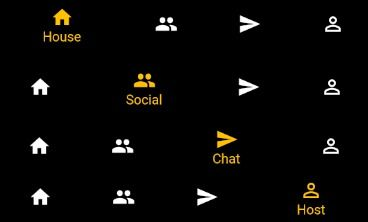
\includegraphics[scale = 0.7]{images/bnb.jpeg}
    \caption{BottomnavigationBar}
\end{figure}

\section{Splash}

\begin{figure}[H]
    \centering
    
\includegraphics[scale = 0.4]{images/splash.png}
    \caption{Slash Screen}
\end{figure}
The Splash Screen welcomes the user when the application is starting; meanwhile it restores the state of the application or loads the default one.\\

\section{Login/SignUp}

\begin{figure}[H]
    \centering
    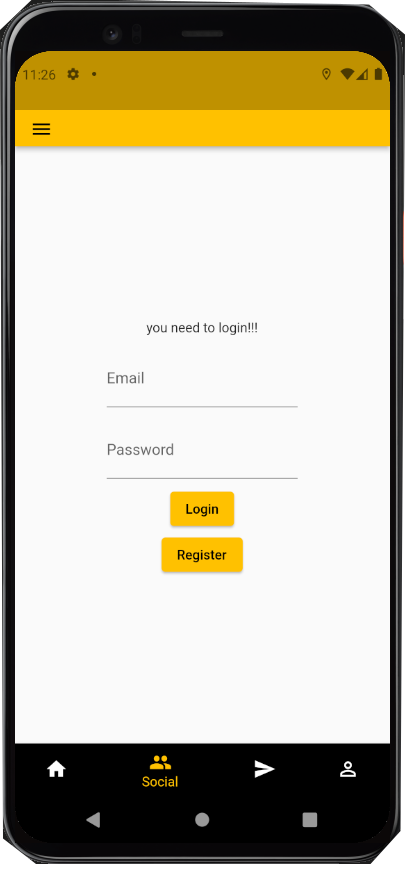
\includegraphics[scale = 0.4]{images/loginsignup.png}
    \caption{Login Screen}
\end{figure}
The login screen is composed by a form in which the users inserts the credentials to log into
the system. If users are not yet registered, they can sign up.\\

\section{House Screen}

\begin{figure}[H]
    \centering
    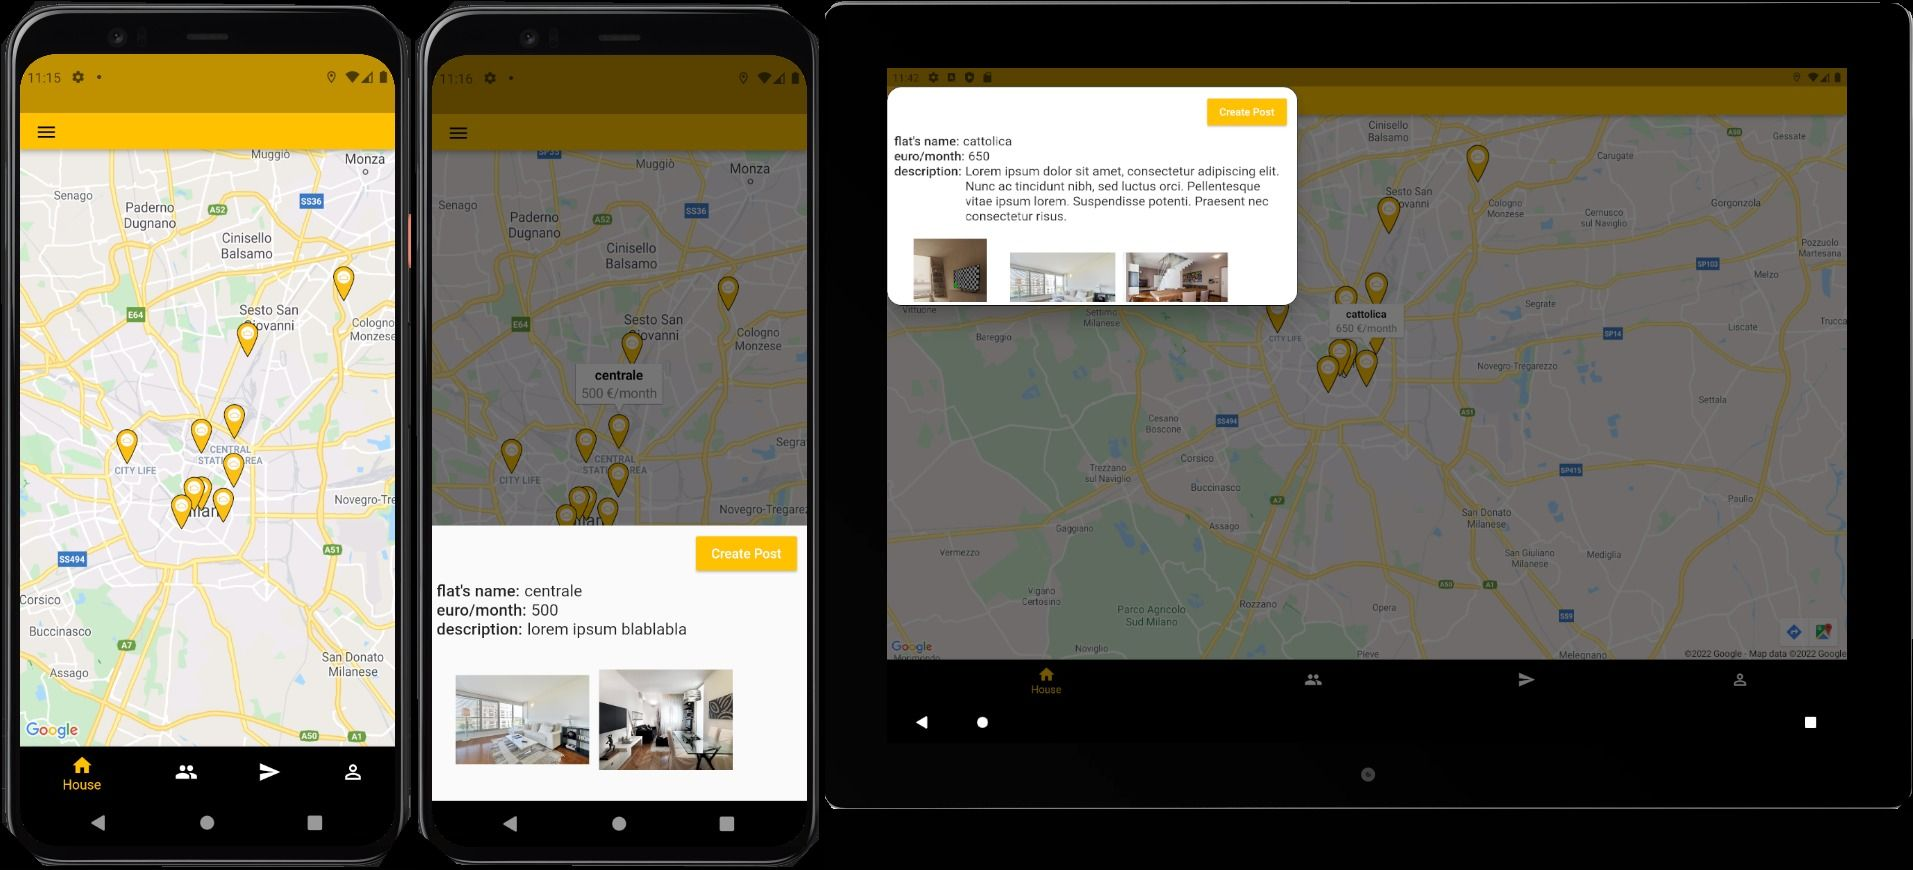
\includegraphics[scale = 0.25]{images/housescreen.jpeg}
    \caption{House Screen and apartment details on smartphone and tablet}
\end{figure}
The House Screen is the first screen that users see once the application is loaded. Users can click on any marker to see further information about houses. After clicking, users can see two different screen layouts according to the device they are using.\\

\section{Social Screen}

\begin{figure}[H]
    \centering
    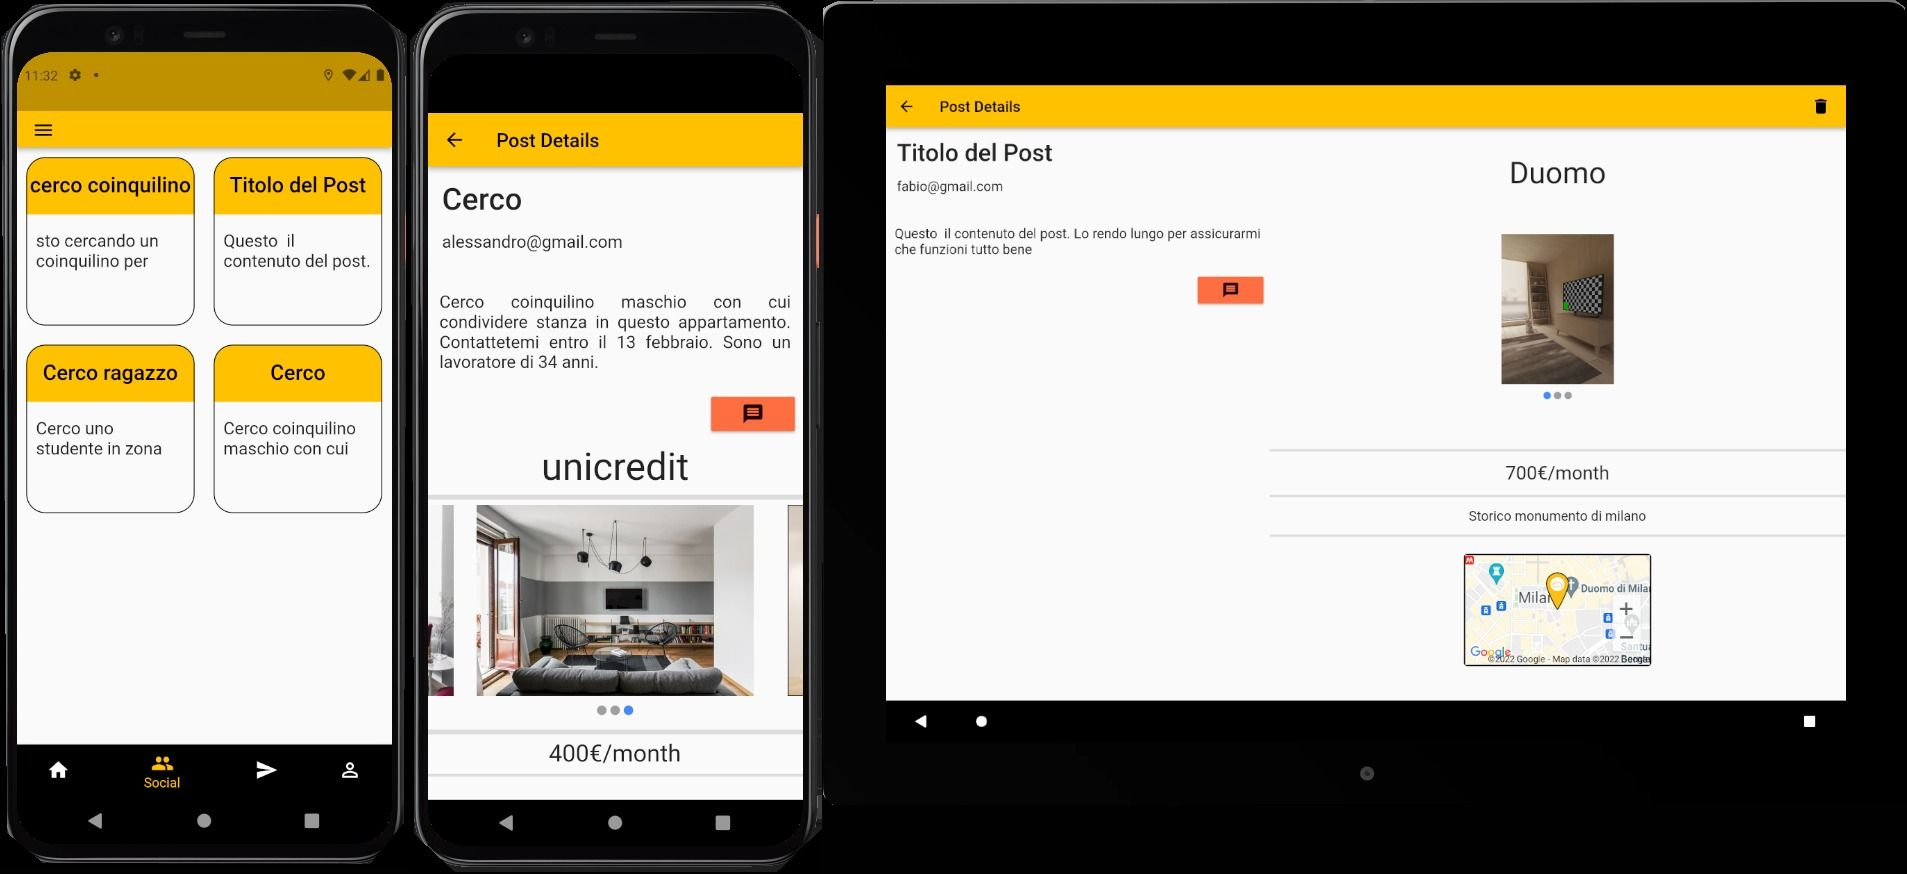
\includegraphics[scale = 0.25]{images/postscreen.jpeg}
    \caption{Social Screen and post details on smartphone and tablet}
\end{figure}
The social screen is organized as a bulletin board with different post-it attached to it. If users click on a post they can see further information in different layouts for smartphone and tablet.\\

\section{Chat Screen}

\begin{figure}[H]
    \centering
    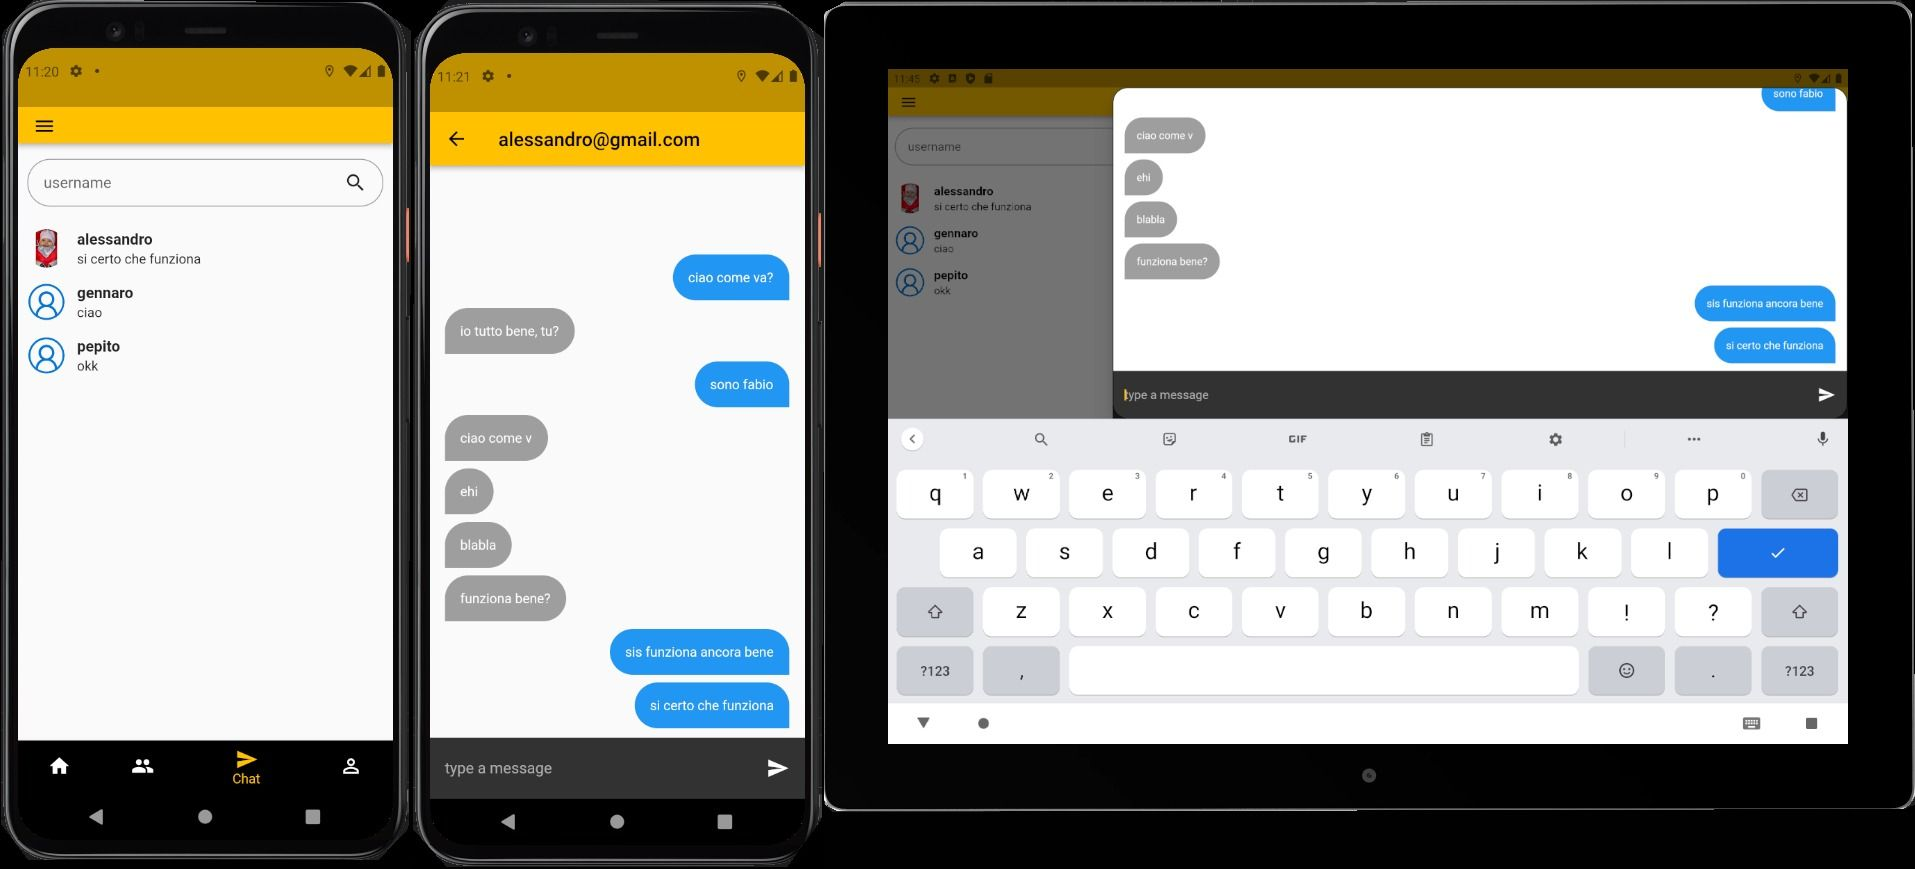
\includegraphics[scale = 0.25]{images/chatscreen.jpeg}
    \caption{Chat Screen and single chat on smartphone and tablet}
\end{figure}
Chat screen is a list of all chats started by the logged in user. When users click on a chat, the chat is displayed with a different layout according to the device they are using.\\

\section{Host Screen}

\begin{figure}[H]
    \centering
    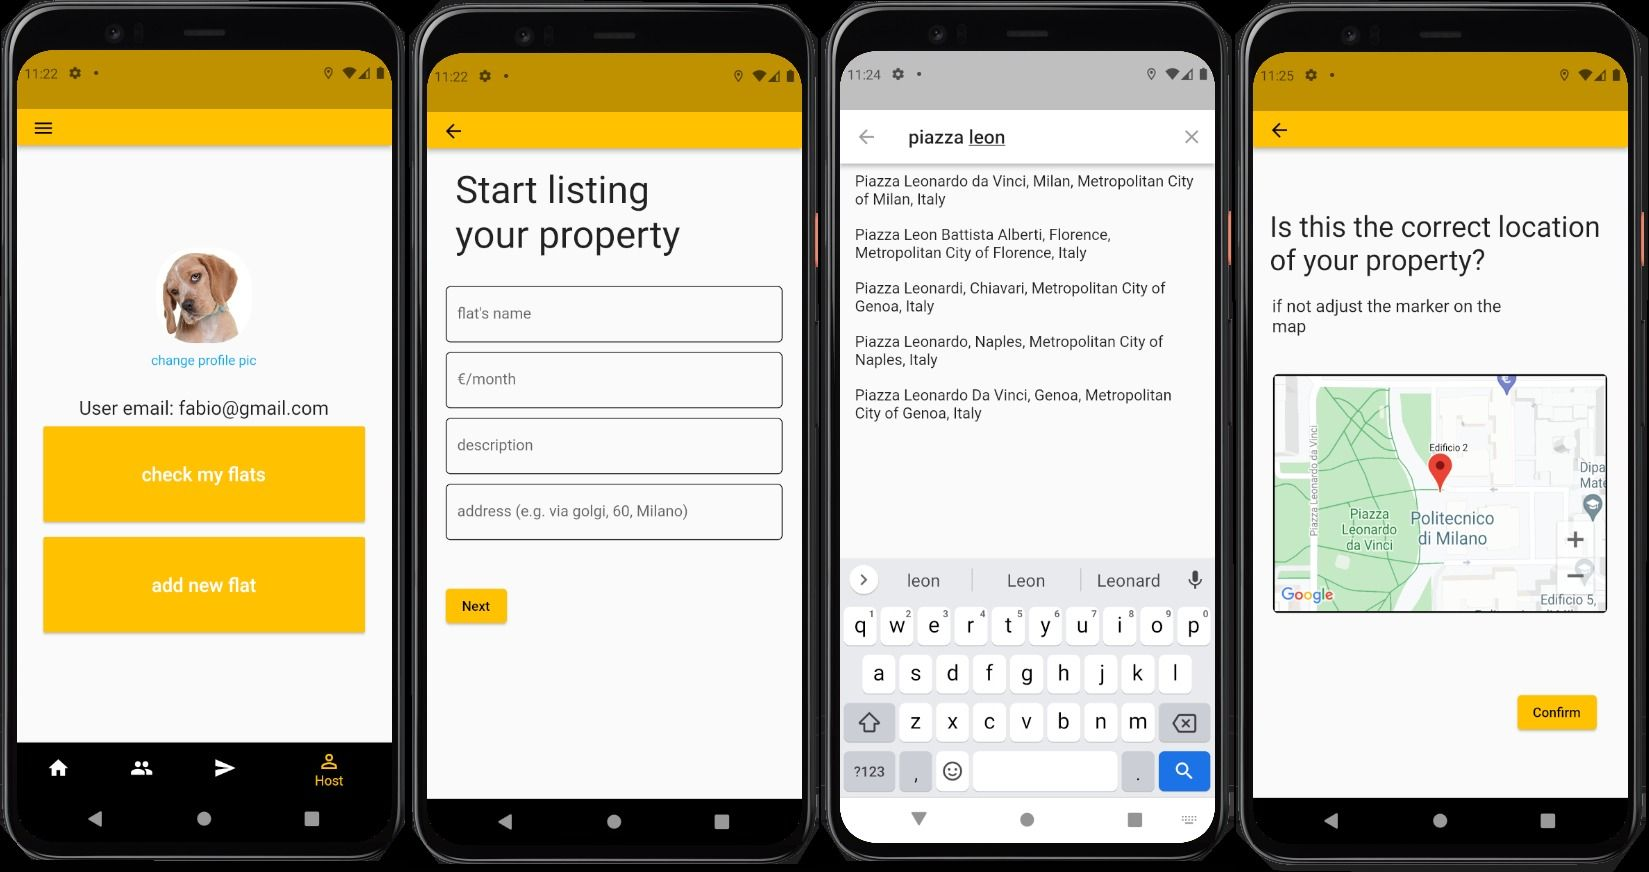
\includegraphics[scale = 0.25]{images/hostscreen.jpeg}
    \caption{Host screen, add house and autocomplete screen}
\end{figure}
The Host screen has two main buttons: the first allows to see all his properties and the second one allows to add a new property. When clicking on "add" button, a new screen appears together with a form in which the users inserts the details. When the host inserts the address, the autocomplete screen appears. At the end of the process, the host will be requested to confirm or adjust the location moving the marker in a small map.\\